\chapter{Running PyLith}

\section{Supported Finite Elements}

PyLith currently only supports the 4-node linear tetrahedral and
8-node linear hexahedral elements. The node ordering must follow the
convention shown in figures~\ref{fig:tet4} and~ref{fig:hex8}.

\begin{figure}[htbp]
  \begin{center}
    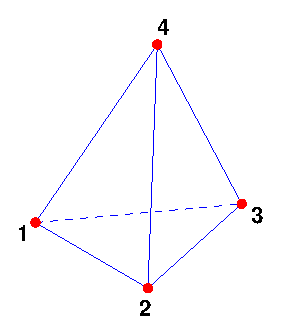
\includegraphics{figs/tet4}
    \caption{Linear tetrahedral finite element.}
    \label{fig:tet4}
  \end{center}
\end{figure}

\begin{figure}[htbp]
  \begin{center}
    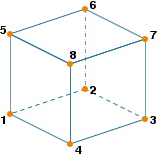
\includegraphics{figs/hex8}
    \caption{Linear hexahedral finite element.}
    \label{fig:hex8}
  \end{center}
\end{figure}

\section{Input Files}

PyLith gets its input from a variety of files. Most of these are
associated with different kinds of boundary conditions. As a result
only six files are required. The remaining files are only used when
the associated boundary condition is used. See
Appendix~\ref{app:file:formats} for a detailed discussion of the file
formats.

The first step in the simulation process involves partitioning the
mesh among the processors. In this phase, PyLith reads in the entire
mesh and then writes out processor specific pieces with one file for
each processor. The filenames for these follow the convention
\filename{xx.PROC.ext} where \filename{PROC}
refers to the processor number and \filename{xx.ext} was the
original filename. This procedure is applied to files with the
following extensions: \filename{coord},
\filename{connect}, \filename{split}, and
\filename{bc}.

The remaining files provide information common to all processors. As a
result, the user must create copies of each one for each of the
processors. By default PyLith expects the names of these files to
follow the same form, \filename{xx.PROC.ext}. Setting up this naming
scheme is most easily done using symbolic links or copying files to
local directories on each machine using a shell script that starts a
simulation. See \filename{runbm.py} in
section~\ref{sec:tutorial:reversenog} for a simple example. You can
also choose your own filename template by setting the appropriate
command-line argument. See ~\ref{sec:commandline:args} for more
information.


\subsection{Required Input Files}

The required input files define the finite-element mesh, boundary
conditions, time step information, output, and material properties.

\begin{description}
\item[\filename{xx.coord}] Coordinates of finite-element vertices.
\item[\filename{xx.connect}] Topology and material information for
  the finite-element mesh.
\item[\filename{xx.bc}] Boundary conditions at vertices on external
  boundaries.
\item[\filename{xx.time}] Time stepping information.
\item[\filename{xx.statevar}] State variables to be output for the
  elastic and (time-dependent) viscoelastic solution.
\item[\filename{xx.prop}] Properties for each material.
\end{description}

\subsection{Optional Input Files}

The optional input files are only read when a file exists matching the
name of an input file PyLith expects to read.  Note that explicit
filenames for each of the files can be specified using command-line
arguments as discussed in section~\ref{sec:commandline:args}.

\begin{description}
\item[\filename{xx.fuldat}] Time steps for which full output is
  requested.
\item[\filename{xx.split}] Dislocation boundary condition information
  (implemented using split nodes).
\item[\filename{xx.skew}] Local coordinate rotation information for
  boundary conditions.
\item[\filename{xx.keyval}] File for changing default parameters.
\item[\filename{xx.wink}] Winkler spring element boundary condition
  information. {\em Not yet tested.}
\item[\filename{xx.hist}] Time histories for split node and Winkler boundary
  conditions (if necessary). {\em Not yet
    tested.}
\end{description}

\section{Command-line Arguments}
\label{sec:commandline:args}

In general, PyLith's command-line arguments fall into three
categories: MPI settings, Pyre properties and facilities, and PETSc
settings.

If using the MPICH implementation of the Message Passing Interface
(MPI), as is done for the CIG distributed binaries, the synopsis for
running PyLith is \\
\command{mpirun} -np \replaceable{NPROCS} pylith3dapp.py
\replaceable{PyLith settings} \replaceable{PETSc settings}

\subsection{MPI Settings}

\begin{warning}
  This section applies only to PyLith compiled using the MPICH
  implementation of the Message Passing Interface (MPI).
\end{warning}


The MPI settings define how many processors are used and other
parallel processing parameters. The number of processors is specified
using \option{-np NPROCS}, where \replaceable{NPROCS} corresponds to
the number of processors.

\subsection{Properties and Facilities}

PyLith gathers many simulation parameters and settings using Pyre
properties and facilities. Properties correspond to simple settings in
the form of strings, integers, and real numbers. Facilities
corresponds to software modules. Both facilities and properties have
default values provided, so you only need to set values when you want
to deviate from the default behavior. Unless you write a module that
extends PyLith's functionality, you will never need to change any of
the facilities from the defaults.

In the current version of PyLith, all of the properties are associated
with the scanner component. You can get a list of all of these
properties along with a description of what they do by running PyLith
with the \option{--scanner.help-properties} command-line argument.

\begin{figure}
  \begin{center}
    \begin{screen}
      mpirun -np \replaceable{1} pylith3dapp.py\\
      --scanner.help-properties --scanner.asciiOutput=\replaceable{none}\\
      --scanner.title=\replaceable{"My simulation"}
    \end{screen}
    \caption{Setting scanner properties from the command line.}
  \end{center}
\end{figure}

\subsection{PETSc Settings}

PyLith relies on PETSc for the linear algebra computations. Many of
PETSc options can be set using command-line arguments. The ones of
primary interest in the case of PyLith are shown in
table~\ref{tab:petsc:options}.

\begin{table}[htbp]
  \begin{center}
    \begin{tabular}{ll}
      Argument & Description \\ \hline
      \option{-log\_summary} 
      & Print logging objects and events \\
      \option{-pc\_type \replaceable{bjacobi}}
      & Set preconditioner type to block Jacobi. See PETSc
      documentation for a list of all preconditioner types. \\
      \option{-sub\_pc\_type \replaceable{ilu}}
      & Set preconditioner to incomplete factorization for
      each block. See PETSc documentation for a list of all
      preconditioners. \\
      \option{-ksp\_monitor \replaceable{stdout}}
      & Dump preconditioned residual norm to stdout. If only
      \option{-ksp\_monitor} is given, the default is
      to use stdout. \\
      \option{-ksp\_view}
      & Print linear solver parameters. \\
      \option{-ksp\_rtol \replaceable{1.0e-09}}
      & Tolerance for relative decrease in residual norm
    \end{tabular}
    \caption{Useful command-line arguments for setting PETSc options.}
  \end{center}
\end{table}

\section{Setting Pyre properties using pml files}

PyLith's Pyre properties can also be set using \filename{pml} files.
These are XML files that follow a special Pyre XML schema.

ADD STUFF HERE
